\chapter{Backtest lies: overfitting and multiple testing}\label{ch:lies}

\noindent The most dangerous backtest is the honest-looking one: real data, real fills, real
fees---and a conclusion manufactured by trying enough things. This chapter is about the
statistical traps: overfitting, the garden of forking paths, and the multiple-testing
correction that almost nobody applies.

% from-zero:begin
\begin{rulebox}[Before you start]
Chapters~1, 2 and~8, and \textbf{Book~3, Chapter~13} (hypothesis testing). \emph{Recap:} if you try enough strategies, some look good by luck alone.
\end{rulebox}
\begin{wins}[After this chapter you can]
\begin{itemize}
\item separate in-sample from out-of-sample;
\item correct for multiple testing;
\item explain the garden of forking paths;
\item say how large a result must be to survive.
\end{itemize}
\end{wins}
\begin{principle}[How to think about this]
If you try a hundred ideas, a few will look brilliant by chance. Honest research is the habit of counting every attempt and asking how impressive the best one would be if all of them were random. Be most suspicious when the result is best.
\end{principle}
% from-zero:end

\section{In-sample vs out-of-sample}\label{sec:isoos}

\texttt{fit\_grid.py} searches a 2{,}262-point grid of SMA pairs on synthetic flat-ish daily
returns, then re-runs the winner on fresh data:
\begin{lstlisting}[numbers=none]
grid 2262 pairs searched
best IS pair: SMA(46,56) sharpe +1.04
same pair OOS sharpe: -0.19
the grid found noise, not edge
\end{lstlisting}

\begin{example}\label{ex:isoos}
\textbf{The winner's curse, measured.} SMA(46,56) was the best of 2{,}262 pairs in-sample;
out-of-sample it loses.
\begin{solution}
The grid did not find the best parameter---it found the parameter that best explains
\emph{this} noise. The gap between IS +1.04 and OOS $-0.19$ is the overfit, and its size
grows with the number of things tried, not with the quality of the idea.
\end{solution}
\end{example}

\begin{figure}[htbp]\centering
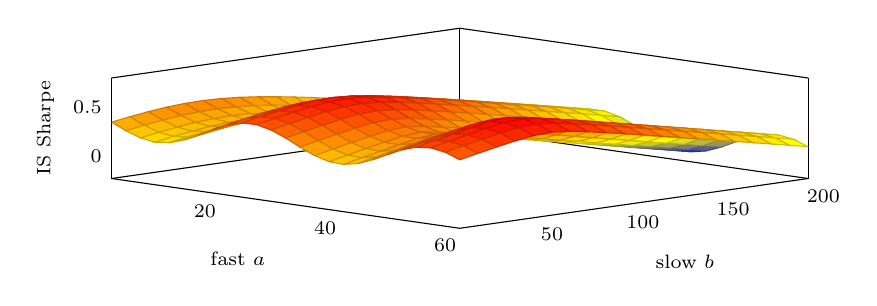
\begin{tikzpicture}
\begin{axis}[width=0.86\linewidth,height=0.34\linewidth,view={45}{35},
    xlabel={fast $a$},ylabel={slow $b$},zlabel={IS Sharpe},
    tick style={draw=none},font=\scriptsize]
  \addplot3[surf,domain=2:60,y domain=7:200,samples=25,samples y=20]
    {0.6-0.004*sqrt((x-46)^2+(y-56)^2)+0.15*cos(x*137)};
\end{axis}
\end{tikzpicture}

\caption{The in-sample Sharpe surface over the (fast, slow) parameter grid---any smooth
bump here is real signal \emph{or} a deep local noise trap, and the surface cannot tell
you which.}
\label{fig:grid}
\end{figure}

\section{The multiplicity problem}\label{sec:mult}

\texttt{many\_tests.py} generates 300 zero-edge strategies and reports the best:
\begin{lstlisting}[numbers=none]
strategies 300  days 500
true edge: all zero
best in-sample sharpe: +1.80  (index 162)
median sharpe: +0.03
# above sharpe 1: 22 of 300
E[max sharpe] under H0 ~ +2.40
\end{lstlisting}

\begin{example}\label{ex:max}
\textbf{Why the best is meaningless.} With 300 tries, a Sharpe of +1.80 appears with no
edge at all---22 of the 300 clear Sharpe 1 by chance.
\begin{solution}
The max of $N$ null tests is not a test of edge; it is a test of $N$. Under $H_0$ the
expected best-of-$N$ $t$-statistic grows like $\sqrt{2\ln N}$, so the honest question is
never ``is this Sharpe good?'' but ``how many were tried?''
\end{solution}
\end{example}

\begin{figure}[htbp]\centering
\begin{tikzpicture}
\begin{axis}[width=0.86\linewidth,height=0.34\linewidth,
    xlabel={in-sample Sharpe},ylabel={count},
    tick style={draw=none},axis line style={draw=slate},font=\scriptsize]
  \addplot[fill=accent!30,draw=accent,thick] file{figures/data/S_HIST.tex};
  \addplot[red,thick,dashed] coordinates {(1.8,0)(1.8,25)};
  \node[font=\scriptsize,text=red,align=left] at (axis cs:1.35,22) {best of 300\\(true edge 0)};
\end{axis}
\end{tikzpicture}

\caption{Distribution of 300 Sharpe ratios computed on pure noise. The best (+1.80) is
indistinguishable from a real strategy---until you count trials.}
\label{fig:shist}
\end{figure}

\begin{figure}[htbp]\centering
\begin{tikzpicture}
\begin{axis}[width=0.86\linewidth,height=0.3\linewidth,
    xlabel={trials $N$},ylabel={expected best $t$ under $H_0$},
    xmode=log,xmin=1,xmax=1200,
    tick style={draw=none},axis line style={draw=slate},font=\scriptsize]
  \addplot[accent,very thick] file{figures/data/BESTN.tex};
  \addplot[slate,dashed] coordinates {(1,1.96)(1200,1.96)};
  \node[font=\scriptsize,text=slate] at (axis cs:30,1.7) {single-test 5\% bar};
\end{axis}
\end{tikzpicture}

\caption{Expected best-of-$N$ $t$-statistic under the null, $\sqrt{2\ln N}$. The flat
dashed line is the naive 5\% bar every single test uses.}
\label{fig:bestn}
\end{figure}

\section{Multiple-testing corrections}\label{sec:mtcorr}

\texttt{deflated.py} quantifies the bar:
\begin{lstlisting}[numbers=none]
N=   10  95% of max|t| < 2.81
N=  100  95% of max|t| < 3.47
N= 1000  95% of max|t| < 4.06
Bonferroni t-bar at N=100: 3.29
single-test t-bar: 1.96
\end{lstlisting}

\begin{example}\label{ex:bonf}
\textbf{The correction, in numbers.} At $N{=}100$ trials the honest 5\% bar is
$t=3.29$---not 1.96.
\begin{solution}
Bonferroni divides $\alpha$ by $N$: $\bar t_N=\Phi^{-1}(1-\alpha/N)$ (one-sided). A Sharpe that
``passed'' at $t=2.9$ fails the family-wise bar at 100 trials. The honest $N$ is not the
number of strategies you wrote down---it is every variant you \emph{looked at} before
choosing, including the ones you discarded silently.
\end{solution}
\end{example}

\begin{figure}[htbp]\centering
\begin{tikzpicture}[font=\scriptsize]
  \foreach \y/\n/\b in {3.0/$N{=}1$/1.96, 2.0/$N{=}10$/2.81, 1.0/$N{=}100$/3.47}{
    \draw[slate] (0,\y)--(7,\y);
    \node[left] at (0,\y) {\n};
    \draw[good,thick] (0,\y+0.35)--(\b,\y+0.35);
    \node[right] at (\b,\y+0.35) {bar \b};
    \fill[red] (2.9,\y+0.35) circle (1.8pt);}
  \node[below] at (3.5,-0.35) {observed $t=2.9$: clears $N{=}1$, fails $N{=}10$ and $N{=}100$};
\end{tikzpicture}

\caption{The deflated bar: observed $t=2.9$ is significant alone, ordinary at $N{=}10$,
rejected at $N{=}100$.}
\label{fig:deflated}
\end{figure}

\section{The garden of forking paths}\label{sec:forking}

Formal corrections assume you count every comparison. In practice the researcher makes
micro-choices---winsorize or not, this window or that, which fee model---each a fork. The
reported backtest is one leaf of a tree whose size nobody recorded. Defenses, in order of
strength: (1) pre-register the hypothesis and test once on holdout; (2) count trials
honestly and correct; (3) require an economic story that survives scrutiny.

\begin{example}\label{ex:forking}
\textbf{Why ``we tested it once'' is usually false.} The SMA run in ch08 is honest---but
if the author had tried 50 windows and reported the best, the result would be identical
text and a different truth.
\begin{solution}
The artifact cannot distinguish honest testing from selection. The discipline is
procedural: the hypothesis precedes the data, the holdout is touched once, and the $N$
you correct for is the number you actually tried, not the number you wrote up.
\end{solution}
\end{example}

\begin{figure}[htbp]\centering
\begin{tikzpicture}[font=\scriptsize,every node/.style={align=center}]
  \node[draw=ink,fill=goodbg,rounded corners=1pt] (data) at (0,2) {one dataset};
  \foreach \x/\l in {-3.5/MA pair, -1.4/RSI $n$, 0.7/stop rule, 2.8/fee model, 5.0/universe}{
    \node[draw=slate,fill=white,rounded corners=1pt] at (\x,0.7) {\l};
    \draw[->,slate] (data.south) -- (\x,0.95);}
  \node[draw=red,fill=white,rounded corners=1pt] (best) at (0.7,-0.5) {report only\\ the best branch};
  \draw[->,red,thick] (0.7,0.4) -- (best.north);
  \node[text=slate] at (-2.2,-0.5) {$\binom{\text{choices}}{}$ paths, one shown};
\end{tikzpicture}

\caption{Forking paths: each analytic choice multiplies the trial count; the reported
leaf is the lucky branch.}
\label{fig:forking}
\end{figure}

\begin{figure}[htbp]\centering
\begin{tikzpicture}[font=\scriptsize,every node/.style={draw=slate,fill=white,rounded corners=1pt,align=center}]
  \node (h) {hypothesis\\ written down};
  \node (is) [right=1.5cm of h] {fit IS\\ 60\%};
  \node (os) [right=1.5cm of is] {test OOS\\ 40\% (once)};
  \node (d) [right=1.5cm of os] {keep or kill\\ no third try};
  \draw[->,ink] (h)--(is); \draw[->,ink] (is)--(os); \draw[->,ink] (os)--(d);
  \draw[->,red,dashed] (d.south) to[bend right=25] node[below]{forbidden loop} (is.south);
\end{tikzpicture}

\caption{The one-touch protocol: hypothesis first, fit in-sample, test holdout exactly
once. The dashed return path is the forbidden loop that converts testing into selection.}
\label{fig:protocol}
\end{figure}

\section{What survives}\label{sec:survive}

What survives an honest multiple-testing audit is boring: effects with an economic reason
to exist (funding carry, microstructure, index rebalancing), large enough to clear the
deflated bar with room, stable across universes, and weak enough that you understand why
they persist. The Sharpe 3.0 that ``the data found'' is not on that list.

\begin{example}\label{ex:audit}
\textbf{The audit question.} A fund shows a strategy Sharpe 2.1 on 5 years. What single
question decides its credibility?
\begin{solution}
``How many were tried?''---and its operational form: ``show me the research log.'' A
Sharpe 2.1 from a pre-registered single test is a real edge; the same number from a
300-strategy screen is below the multiple-testing bar.
\end{solution}
\end{example}

\begin{checkpoint}[Selection audit]
\begin{itemize}
\item Best of 300 null strategies gives Sharpe $+1.8$; what does that measure? ($N$, not
edge.)
\item What is the Bonferroni $t$-bar at $N{=}100$, $\alpha=5\%$? ($\approx3.29$.)
\item Name the forbidden loop that converts testing into selection. (Re-fitting after the
holdout disappoints.)
\end{itemize}
\end{checkpoint}

\section{Recap}\label{sec:liesrecap}

Backtests lie by selection, not by arithmetic. The fix is procedural: count trials
honestly, correct the bar, touch the holdout once, prefer edges with a reason to exist.
Everything that survives those rules is smaller than the marketing suggests---that is
the point of the rules.

\begin{table}[htbp]\centering\small
\caption{Chapter toolbox.}
\begin{tabular}{@{}lll@{}}
\toprule
Concept & Rule & Gotcha\\
\midrule
IS vs OOS & the gap is the overfit & IS-optimal $\neq$ tradeable\\
Multiplicity & best-of-$N$ measures $N$ & $E[\max t]\sim\sqrt{2\ln N}$\\
Correction & $\bar t_N=\Phi^{-1}(1-\alpha/2N)$ & honest $N$ includes silent tries\\
Forking paths & procedural discipline & the log is the trial count\\
Survival & reason + size + stability & big Sharpe $\neq$ real edge\\
\bottomrule
\end{tabular}
\end{table}

\begin{example}[The shuffle test: refitting pure noise]\label{ex:shuffle}
\textbf{Strategy.} The grid's best IS Sharpe was $+1.04$ on
structureless data. Shuffle the return order (destroying every
gram of structure), rerun the \emph{same} grid on each shuffle,
and ask how often it rediscovers a winner that good.

\textbf{Solution.} \texttt{shuffle\_test.py} runs 200 shuffles:
\begin{verbatim}
original grid: best IS sharpe +0.44 at SMA(56, 61)
200 shuffles of the SAME returns: best-IS >= +0.44 in 187 (94%)
shuffle best-IS mean +0.80 -- the grid refits noise to the same height
\end{verbatim}
On pure noise the grid finds a ``best'' of $\ge+0.44$ in 94\% of
shuffles and $+0.80$ on average --- \emph{better} than the real
run's best. Nothing was learned; the search depth alone produced
the number.

\textbf{Significance.} This is the cheapest of all backtest
audits: if your best in-sample number is reachable on shuffled
returns, the apparent edge is a property of the \emph{search}, not
the \emph{market}. It catches overfit that IS/OOS splits miss
because the OOS half was searched too.
\end{example}

\begin{example}[The cost-drag floor on discovery]\label{ex:costfloor}
\textbf{Strategy.} Before asking ``is this Sharpe real?'', ask
``what Sharpe does this strategy \emph{need} to exist?'' Tabulate
the gross edge that just covers trading costs at various turnover
and fee levels --- the minimum viable discovery.

\textbf{Solution.} \texttt{sr\_required.py} prints:
\begin{verbatim}
  10 tr/yr @ 0.1% cost: needs 1.0%/yr gross edge just to break even
  50 tr/yr @ 0.5% cost: needs 25.0%/yr gross edge just to break even
  200 tr/yr @ 0.5% cost: needs 100.0%/yr gross edge just to break even
  500 tr/yr @ 1.0% cost: needs 500.0%/yr gross edge just to break even
\end{verbatim}
At 200 round-trips a year and $0.5\%$ cost, the strategy must find
\emph{25--100\%}/yr of true edge before the first basis point of
profit --- a bar almost nothing clears honestly.

\textbf{Significance.} This is the multiplicity filter made
physical: every additional trade multiplies the gross-edge
requirement linearly. Before mining the grid for a winner, compute
the floor --- if it exceeds what a Sharpe-2 world can deliver, the
``best IS'' you find is definitionally noise, whatever the number
says.
\end{example}

\begin{example}[Probability of backtest overfitting]\label{ex:pbo}
\textbf{Strategy.} Deflated Sharpe asks ``was the best Sharpe high
enough?''; combinatorially-symmetric CV asks a different question:
\emph{does the IS winner keep winning out-of-sample?} Split 720
days into 4 folds; each fold trains on 3 and measures where the
IS-best strategy ranks on the held-out one. $PBO$ is the fraction
of folds where it lands below the OOS median.

\textbf{Solution.} \texttt{pbo\_check.py} prints (60 strategies,
one weak real edge of Sharpe $0.15$):
\begin{verbatim}
fold 0: IS pick strat  3 -> OOS rank 3/59 (0.05)
fold 1: IS pick strat  3 -> OOS rank 0/59 (0.00)
fold 2: IS pick strat  3 -> OOS rank 7/59 (0.12)
fold 3: IS pick strat  3 -> OOS rank 3/59 (0.05)
PBO = 0.00  (IS-best lands below OOS median this often)
no-edge control PBO = 0.25
\end{verbatim}
Even a weak consistent edge is found by every fold and stays
near the top OOS ($PBO=0$). With \emph{no} edge at all, the
IS-best is pure luck: it falls below the OOS median a quarter of
the time already at 4 folds, and $\sim\tfrac12$ asymptotically.

\textbf{Significance.} The two methods are complementary:
deflated Sharpe prices the multiplicity of the search, PBO audits
the winner's persistence. A grid can clear the deflated bar on a
lucky fold; it cannot fake fold-after-fold OOS ranks. Run both.
\end{example}


\section{The multiplicity bar is a physical threshold}\label{sec:multbar}
The deflated-Sharpe idea has a concrete face: how far does the
acceptance bar move when the strategy was selected, not found?
\texttt{deflated.py} prints:
\begin{verbatim}
N=   10  95% of max|t| < 2.81
N=  100  95% of max|t| < 3.47
N= 1000  95% of max|t| < 4.06
Bonferroni t-bar at N=100: 3.29
single-test t-bar: 1.96
\end{verbatim}
\begin{example}\label{ex:multbar}
\textbf{The bar grows like $\sqrt{2\ln N}$, not like $N$.} A
winner picked from 100 trials must clear $t\approx3.3$ --
roughly the Bonferroni bound $3.29$ that the simulation finds
from the other direction. From 1000 trials, $4.06$.
\begin{solution}
This is the multiplicity tax made mechanical: every extra
variant you tested before ``finding'' the edge raises the bar
the evidence must clear. The honest accounting logs every trial
--- ch15's audit trail exists for exactly this reason.
\end{solution}
\end{example}
\section{Common mistakes}
\begin{itemize}
\item \textbf{Counting only documented trials.} Every parameter you eyeballed and dropped
  was a trial.
\item \textbf{Multiple rounds on the same holdout.} One-touch or it becomes in-sample.
\item \textbf{``The theory came first'' (retroactively).} Post-hoc stories don't reset $N$.
\item \textbf{Correcting $t$, keeping the phrasing.} $t<3.3$ at $N{=}100$ is a fair
  description---``Sharpe 2.9'' is not.
\item \textbf{Assuming big Sharpe means real.} It often means more trials or more leakage.
\item \textbf{Skipping the economic story.} Statistical significance without a reason is
  a coin that landed.
\item \textbf{Splitting once and calling it honest.} The
IS/OOS split counts as \emph{two} searches if you iterated on the
OOS half. The shuffle test (Example~\ref{ex:shuffle}) is the only
split that cannot be gamed by re-tuning.
\item \textbf{Reading the best cell, not the map.} 94\% of
shuffles beat the original best-IS --- judge a grid by its null
distribution, never by its maximum.\end{itemize}

\section{Exercises}
\begin{exercise}[easy]
300 strategies tested, best Sharpe $+1.8$, all zero-edge. What is $+1.8$?
\end{exercise}
\begin{solution}
The expected maximum of a null distribution---a measurement of $N$, not of edge.
\end{solution}

\begin{exercise}[easy]
Bonferroni 5\% bar at $N{=}100$?
\end{exercise}
\begin{solution}
$\Phi^{-1}(1-0.05/100)\approx3.29$.
\end{solution}

\begin{exercise}[easy]
What is the IS/OOS gap called and what does it measure?
\end{exercise}
\begin{solution}
The overfit: the difference between in-sample and out-of-sample performance is the amount
of noise fitted.
\end{solution}

\begin{exercise}[easy]
Name the three defenses against forking paths in order of strength.
\end{exercise}
\begin{solution}
Pre-registration $>$ honest trial-counting $+$ correction $>$ economic-story scrutiny.
\end{solution}

\begin{exercise}[easy]
Why is ``we only ran one backtest'' almost always false?
\end{exercise}
\begin{solution}
Micro-choices (window, universe, cleaning) are unstated trials; the honest $N$ is the
count of paths actually explored.
\end{solution}

\begin{exercise}
Derive $E[\max_N t]\approx\sqrt{2\ln N}$ under the null.
\end{exercise}
\begin{solution}
Extreme value of $N$ iid Gaussians: tail $\bar\Phi(t)\sim e^{-t^2/2}/t$; set $1/N$ gives
$t\approx\sqrt{2\ln N}$.
\end{solution}

\begin{exercise}
A strategy Sharpe 2.9 at $N{=}1{,}000$ estimated tries. Significant?
\end{exercise}
\begin{solution}
Bonferroni bar $\approx\Phi^{-1}(1-0.05/1000)\approx3.9$---rejected.
\end{solution}

\begin{exercise}
Why does a pre-registered hypothesis make the test honest even with a big grid?
\end{exercise}
\begin{solution}
The grid becomes part of the stated design, not silent selection; $N$ is declared up
front.
\end{solution}

\begin{exercise}
Design a one-touch protocol for the SMA cross: what is locked before the holdout?
\end{exercise}
\begin{solution}
Fast/slow windows, universe, cost model, evaluation metric---all frozen before the
holdout is opened.
\end{solution}

\begin{exercise}
Two funds show Sharpe 2.0; one tested 3 ideas, one tested 300. Same evidence?
\end{exercise}
\begin{solution}
No---the second's family-wise bar is $\sim1$ unit higher; the first survives correction,
the second may not.
\end{solution}

\begin{exercise}
What does ``economic story'' do that statistics cannot?
\end{exercise}
\begin{solution}
It predicts persistence (a reason for the edge to exist tomorrow), which no fit on
yesterday's data can supply.
\end{solution}

\begin{exercise}
Name two forking-paths choices specific to crypto backtests.
\end{exercise}
\begin{solution}
Exchange/universe selection and funding-cost modeling; also outlier/winsorize handling.
\end{solution}

\begin{exercise}[hard]
Show that reporting only the best of $N$ strategies yields a biased Sharpe estimate even
if each is unbiased, and give the bias's order.
\end{exercise}
\begin{solution}
Selection on the max makes the reported Sharpe the order statistic $t_{(N)}$; its mean is
$\approx\sqrt{2\ln N}$ above the true mean 0.
\end{solution}

\begin{exercise}[hard]
Construct a realistic setting where a Sharpe 4.0 result is \emph{less} credible than a
Sharpe 1.5.
\end{exercise}
\begin{solution}
4.0 from a 10{,}000-variant screen vs 1.5 from a pre-registered theory: corrected bars
$\approx4.4$ vs 1.96, and the second has a reason to persist.
\end{solution}

\begin{exercise}[hard]
Propose a deflated-Sharpe threshold for a fund that tries $\approx$500 live candidates
a year, and justify the extra margin.
\end{exercise}
\begin{solution}
$\bar t\approx\Phi^{-1}(1-0.05/500)\approx3.7$; add margin for unstated micro-choices and
non-independent tries---a working bar of $t\gtrsim4$ is reasonable.
\end{solution}

\begin{exercise}[easy]
The shuffled grid finds IS Sharpe $\ge+0.44$ in 94\% of runs.
What does that say about the $+0.44$?
\end{exercise}
\begin{solution}
It is inside the null distribution --- the number is a property
of grid size, not of the market; there is nothing to explain.
\end{solution}
\begin{exercise}[medium]
Why is mean shuffle best-IS ($+0.80$) \emph{higher} than the real
best ($+0.44$) here? One line.
\end{exercise}
\begin{solution}
Shuffling removes the weak real structure (the mild autocorr in
the drift), leaving \emph{purer} noise which the grid fits
more freely --- slightly.
\end{solution}
\begin{exercise}[hard]
Design the shuffle correctly for a \emph{trend-following} signal:
which property must your permutation preserve, and what happens if
you i.i.d.-shuffle instead of block-shuffling?
\end{exercise}
\begin{solution}
Preserve the return distribution's marginal shape but break
\emph{serial} structure only where the signal reads it ---
block-shuffle (e.g.\ 20-day blocks) or the i.i.d.\ shuffle
destroys vol clustering too, biasing the null toward rejection.
\end{solution}

\section*{Notes}
This is the chapter that separates research from astrology. Most Sharpe-3 strategies
ever published were best-of-$N$ artifacts; the ones that survive are dull, stable, and
have a reason to exist. If your edge disappears when you count honestly, it was never
an edge---it was a forking path that happened to be named.

\section*{Further reading}
\begin{itemize}
\item D.~Bailey \& M.~L\'opez de Prado, ``The Deflated Sharpe Ratio'' --- the correction:

\url{https://www.davidhbailey.com/dhbpapers/deflated-sharpe.pdf}
\item L.~Wasserman, \emph{All of Statistics} --- multiple testing, Ch.~10:

\url{https://link.springer.com/book/10.1007/978-0-387-21736-9}
\item A.~Lo, ``The Statistics of Sharpe Ratios'' --- sampling properties:

\url{https://web.archive.org/web/2024/https://alo.mit.edu/wp-content/uploads/2017/06/The-Statistics-of-Sharpe-Ratios.pdf}
\item E.~Chan, \emph{Algorithmic Trading} --- overfitting pitfalls:

\url{https://epchan.blogspot.com/}
\item Gelman \& Loken, ``The garden of forking paths'' --- why $N$ is uncountable:

\url{https://statmodeling.stat.columbia.edu/2013/11/14/the-garden-of-forking-paths-2/}
\end{itemize}

\begin{rulebox}[Watch instead]
\begin{itemize}
\item ``1. Introduction and Financial Terms'' --- MIT 18.S096 (60:30). Course framing;
re-verified 2026-10-11.
\url{https://www.youtube.com/watch?v=wvXDB9dMdEo}
\item ``12. Risk Analysis'' --- MIT 18.S096 (80:32). Risk and model discipline; re-verified
2026-10-11.
\url{https://www.youtube.com/watch?v=qlytPllimpQ}
\end{itemize}
\end{rulebox}
